\documentclass[]{article}
\usepackage{lmodern}
\usepackage{amssymb,amsmath}
\usepackage{ifxetex,ifluatex}
\usepackage{fixltx2e} % provides \textsubscript
\ifnum 0\ifxetex 1\fi\ifluatex 1\fi=0 % if pdftex
  \usepackage[T1]{fontenc}
  \usepackage[utf8]{inputenc}
\else % if luatex or xelatex
  \ifxetex
    \usepackage{mathspec}
  \else
    \usepackage{fontspec}
  \fi
  \defaultfontfeatures{Ligatures=TeX,Scale=MatchLowercase}
\fi
% use upquote if available, for straight quotes in verbatim environments
\IfFileExists{upquote.sty}{\usepackage{upquote}}{}
% use microtype if available
\IfFileExists{microtype.sty}{%
\usepackage{microtype}
\UseMicrotypeSet[protrusion]{basicmath} % disable protrusion for tt fonts
}{}
\usepackage[margin=1in]{geometry}
\usepackage{hyperref}
\hypersetup{unicode=true,
            pdftitle={36-315 Homework 01, Spring 2019},
            pdfauthor={Eu Jing Chua},
            pdfborder={0 0 0},
            breaklinks=true}
\urlstyle{same}  % don't use monospace font for urls
\usepackage{color}
\usepackage{fancyvrb}
\newcommand{\VerbBar}{|}
\newcommand{\VERB}{\Verb[commandchars=\\\{\}]}
\DefineVerbatimEnvironment{Highlighting}{Verbatim}{commandchars=\\\{\}}
% Add ',fontsize=\small' for more characters per line
\usepackage{framed}
\definecolor{shadecolor}{RGB}{248,248,248}
\newenvironment{Shaded}{\begin{snugshade}}{\end{snugshade}}
\newcommand{\AlertTok}[1]{\textcolor[rgb]{0.94,0.16,0.16}{#1}}
\newcommand{\AnnotationTok}[1]{\textcolor[rgb]{0.56,0.35,0.01}{\textbf{\textit{#1}}}}
\newcommand{\AttributeTok}[1]{\textcolor[rgb]{0.77,0.63,0.00}{#1}}
\newcommand{\BaseNTok}[1]{\textcolor[rgb]{0.00,0.00,0.81}{#1}}
\newcommand{\BuiltInTok}[1]{#1}
\newcommand{\CharTok}[1]{\textcolor[rgb]{0.31,0.60,0.02}{#1}}
\newcommand{\CommentTok}[1]{\textcolor[rgb]{0.56,0.35,0.01}{\textit{#1}}}
\newcommand{\CommentVarTok}[1]{\textcolor[rgb]{0.56,0.35,0.01}{\textbf{\textit{#1}}}}
\newcommand{\ConstantTok}[1]{\textcolor[rgb]{0.00,0.00,0.00}{#1}}
\newcommand{\ControlFlowTok}[1]{\textcolor[rgb]{0.13,0.29,0.53}{\textbf{#1}}}
\newcommand{\DataTypeTok}[1]{\textcolor[rgb]{0.13,0.29,0.53}{#1}}
\newcommand{\DecValTok}[1]{\textcolor[rgb]{0.00,0.00,0.81}{#1}}
\newcommand{\DocumentationTok}[1]{\textcolor[rgb]{0.56,0.35,0.01}{\textbf{\textit{#1}}}}
\newcommand{\ErrorTok}[1]{\textcolor[rgb]{0.64,0.00,0.00}{\textbf{#1}}}
\newcommand{\ExtensionTok}[1]{#1}
\newcommand{\FloatTok}[1]{\textcolor[rgb]{0.00,0.00,0.81}{#1}}
\newcommand{\FunctionTok}[1]{\textcolor[rgb]{0.00,0.00,0.00}{#1}}
\newcommand{\ImportTok}[1]{#1}
\newcommand{\InformationTok}[1]{\textcolor[rgb]{0.56,0.35,0.01}{\textbf{\textit{#1}}}}
\newcommand{\KeywordTok}[1]{\textcolor[rgb]{0.13,0.29,0.53}{\textbf{#1}}}
\newcommand{\NormalTok}[1]{#1}
\newcommand{\OperatorTok}[1]{\textcolor[rgb]{0.81,0.36,0.00}{\textbf{#1}}}
\newcommand{\OtherTok}[1]{\textcolor[rgb]{0.56,0.35,0.01}{#1}}
\newcommand{\PreprocessorTok}[1]{\textcolor[rgb]{0.56,0.35,0.01}{\textit{#1}}}
\newcommand{\RegionMarkerTok}[1]{#1}
\newcommand{\SpecialCharTok}[1]{\textcolor[rgb]{0.00,0.00,0.00}{#1}}
\newcommand{\SpecialStringTok}[1]{\textcolor[rgb]{0.31,0.60,0.02}{#1}}
\newcommand{\StringTok}[1]{\textcolor[rgb]{0.31,0.60,0.02}{#1}}
\newcommand{\VariableTok}[1]{\textcolor[rgb]{0.00,0.00,0.00}{#1}}
\newcommand{\VerbatimStringTok}[1]{\textcolor[rgb]{0.31,0.60,0.02}{#1}}
\newcommand{\WarningTok}[1]{\textcolor[rgb]{0.56,0.35,0.01}{\textbf{\textit{#1}}}}
\usepackage{graphicx,grffile}
\makeatletter
\def\maxwidth{\ifdim\Gin@nat@width>\linewidth\linewidth\else\Gin@nat@width\fi}
\def\maxheight{\ifdim\Gin@nat@height>\textheight\textheight\else\Gin@nat@height\fi}
\makeatother
% Scale images if necessary, so that they will not overflow the page
% margins by default, and it is still possible to overwrite the defaults
% using explicit options in \includegraphics[width, height, ...]{}
\setkeys{Gin}{width=\maxwidth,height=\maxheight,keepaspectratio}
\IfFileExists{parskip.sty}{%
\usepackage{parskip}
}{% else
\setlength{\parindent}{0pt}
\setlength{\parskip}{6pt plus 2pt minus 1pt}
}
\setlength{\emergencystretch}{3em}  % prevent overfull lines
\providecommand{\tightlist}{%
  \setlength{\itemsep}{0pt}\setlength{\parskip}{0pt}}
\setcounter{secnumdepth}{0}
% Redefines (sub)paragraphs to behave more like sections
\ifx\paragraph\undefined\else
\let\oldparagraph\paragraph
\renewcommand{\paragraph}[1]{\oldparagraph{#1}\mbox{}}
\fi
\ifx\subparagraph\undefined\else
\let\oldsubparagraph\subparagraph
\renewcommand{\subparagraph}[1]{\oldsubparagraph{#1}\mbox{}}
\fi

%%% Use protect on footnotes to avoid problems with footnotes in titles
\let\rmarkdownfootnote\footnote%
\def\footnote{\protect\rmarkdownfootnote}

%%% Change title format to be more compact
\usepackage{titling}

% Create subtitle command for use in maketitle
\providecommand{\subtitle}[1]{
  \posttitle{
    \begin{center}\large#1\end{center}
    }
}

\setlength{\droptitle}{-2em}

  \title{36-315 Homework 01, Spring 2019}
    \pretitle{\vspace{\droptitle}\centering\huge}
  \posttitle{\par}
    \author{Eu Jing Chua}
    \preauthor{\centering\large\emph}
  \postauthor{\par}
      \predate{\centering\large\emph}
  \postdate{\par}
    \date{Due Wednesday, Jan 23, 2019 (11:59pm ET) on Canvas}


\begin{document}
\maketitle

\hypertarget{introduction-to-r-rstudio-data-types-and-critiquing-graphics}{%
\subsection{\texorpdfstring{Introduction to \texttt{R}, RStudio, Data
Types, and Critiquing
Graphics}{Introduction to R, RStudio, Data Types, and Critiquing Graphics}}\label{introduction-to-r-rstudio-data-types-and-critiquing-graphics}}

\begin{center}\rule{0.5\linewidth}{\linethickness}\end{center}

\begin{center}\rule{0.5\linewidth}{\linethickness}\end{center}

\textbf{\emph{General instructions for all assignments}}:

\begin{itemize}
\tightlist
\item
  Use this file as the template for your submission. Delete the
  unnecessary text (e.g.~this text, the problem statements, etc). That
  said, keep the nicely formatted ``Problem 1'', ``Problem 2'', ``a.'',
  ``b.'', etc
\item
  Upload a single \texttt{R} Markdown file (named as:
  {[}AndrewID{]}-315-HW01.Rmd -- e.g.~``mneykov-315-HW01.Rmd'') to the
  Homework 01 submission section on Canvas. You do not need to upload
  the .html file.
\item
  The instructor and TAs will run your .Rmd file on their computers.
  \textbf{If your .Rmd file does not knit on our computers, you will be
  automatically be deducted 10 points.}
\item
  Your file should contain the code to answer each question in its own
  code block. Your code should produce plots/output that will be
  automatically embedded in the output (.html) file
\item
  Each answer must be supported by written statements (unless otherwise
  specified)
\item
  Include the name of anyone you collaborated with at the top of the
  assignment
\end{itemize}

\begin{center}\rule{0.5\linewidth}{\linethickness}\end{center}

\begin{center}\rule{0.5\linewidth}{\linethickness}\end{center}

\hypertarget{problem-1}{%
\section{Problem 1}\label{problem-1}}

(12 points)

\textbf{Downloading R and R Studio}:

If you are using your own, personal computer, you will need to download
and install \texttt{R} and RStudio. Follow the instructions here to do
so (be sure to choose the correct operating system, and 64-bit R if
possible/compatible):
{[}\url{https://www.rstudio.com/products/rstudio/download/}{]}

Once you get RStudio open, download the Homework01.Rmd file from Canvas
and open it in RStudio (File / Open\ldots). We recommend using the
Homework01.Rmd file on Canvas as a template for your submission. If you
do, be sure to delete all of the problem statements and additional text,
as these are not necessary to include in your submission.

Notice how the text you write in the .Rmd file shows up in the output
file each time you click ``Knit HTML''.

For more tips/tricks on how to format things in R Markdown, go to
{[}\url{https://www.rstudio.com/wp-content/uploads/2015/02/rmarkdown-cheatsheet.pdf}{]}

\textbf{Customizing the RStudio User Interface}:

The first thing you'll notice is that, in the RStudio window, there are
several panes that contain various things (Console, Help, Environment,
History, Plots, etc).

If you're using Mac, go to RStudio / Preferences / Pane Layout. If
you're using Windows, go to Tools / Global Options. Change the menu
options to arrange the panes as you see fit.

\textbf{In your answer to this problem}, describe your chosen Pane
Layout and give a brief explanation for why you chose this.

Personally, Matey prefers to have:

\begin{itemize}
\tightlist
\item
  Source in its own pane on the top-right-hand side
\item
  Console in it's own pane on the top-left-hand side of the window
\item
  Help on the bottom-left
\item
  Everything else on the bottom-right
\end{itemize}

Click Apply. Now click Appearance and choose an appropriate font, font
size, and theme. Fonts with fixed-width are typically more convenient
for programming.

Click Apply and okay. Minimizing the bottom-left and bottom-right panes
is a nice trick which gives more vertical space to see your code and the
output it's generating.

\textbf{Where is my output file?}

Find where you stored your {[}AndrewID{]}-315-HW01.Rmd file on your
computer.

In the same directory, there should be a file called
{[}AndrewID{]}-315-HW01.html.

Open it. It should automatically open in a browser, and it should
contain the output.

\textbf{Additional Customization Advice} (not required):

\begin{itemize}
\tightlist
\item
  Under Preferences / Code / Display, you might consider adding the
  margin column and setting it to 80 characters, since most style guides
  suggest that you should always keep lines of code at 80 characters or
  less when possible.
\item
  You can set your background color, font, font size, etc under
  Preferences / Appearance. Personally, Matey uses the ``Idle Fingers''
  theme since it's easy on the eyes. Of course, this is strictly a
  personal preference, so you should choose something that you like.
\item
  Under Preferences / Packages, you can opt to change your CRAN mirror
  to the ``Global (CDN) - RStudio'' option, as it is very reliable.
\item
  Under Preferences / Git/SVN, you can configure your version control
  preferences. Although not required, I highly recommend that you use
  Git with RStudio. The interface is easy to use even if you're a
  beginner programmer or Git user.
  \href{https://support.rstudio.com/hc/en-us/articles/200532077-Version-Control-with-Git-and-SVN}{This
  link} and
  \href{https://jennybc.github.io/2014-05-12-ubc/ubc-r/session03_git.html}{this
  link} have more information on this, if you're interested (again, not
  required).
\end{itemize}

I have a setup for working with RMarkdown using Neovim as my main
editor. I use the plugin
\includegraphics{https://github.com/jalvesaq/Nvim-R} to setup the
knitting of PDF/HTML for me with hotkeys. The editor is split vertically
into two, with the top for editting the Rmd file and the bottom as a R
REPL that also outputs the success / failure messages of my knitting.
When knitting to PDF, my PDF viewer Zathura automatically listens for
changes to the PDF and updates accordingly, otherwise I use my regular
browser to see my HTML output.

\begin{center}\rule{0.5\linewidth}{\linethickness}\end{center}

\begin{center}\rule{0.5\linewidth}{\linethickness}\end{center}

\hypertarget{problem-2}{%
\section{Problem 2}\label{problem-2}}

(20 points)

\textbf{Critiquing Graphs}:

Find a graph from the internet (last 7 days -- e.g.~a news article, blog
post, etc) or from an academic journal (last 60 days). Describe and
critique your graph using the suggestions below. In parts (b)-(d), you
do not have to address each bullet below -- these are just suggestions
of things you can discuss when describing/critiquing your graph.

\begin{enumerate}
\def\labelenumi{\alph{enumi}.}
\tightlist
\item
  (5 points) \textbf{Include the graph in your assignment}. Two choices
  here:
\end{enumerate}

\begin{itemize}
\tightlist
\item
  embed the graph/image in the .html file (see below for instructions)
  and submit it along with your other files on Canvas, or
\item
  include a link to the graph in your answer to this question.
\end{itemize}

\begin{enumerate}
\def\labelenumi{\alph{enumi}.}
\setcounter{enumi}{1}
\tightlist
\item
  (5 points) \textbf{Describe the graph}.
\end{enumerate}

\begin{itemize}
\tightlist
\item
  What does the graph show?
\item
  What variables are plotted on the axes, via color, or via other
  features of the graph?
\item
  \textbf{What is the main result of the graph?}
\end{itemize}

\begin{enumerate}
\def\labelenumi{\alph{enumi}.}
\setcounter{enumi}{2}
\tightlist
\item
  (5 points) \textbf{Critique the graph}.
\end{enumerate}

\begin{itemize}
\tightlist
\item
  Does the graph do a good job of achieving its goals?
\item
  Does the graph use an unnecessary amount of data ink?
\item
  Does the graph distort the actual effect/data/relationship?
\item
  What are the strengths and weaknesses (if any) of the graphic?
\item
  What would you change (if anything) about this graphic?
\end{itemize}

\begin{enumerate}
\def\labelenumi{\alph{enumi}.}
\setcounter{enumi}{3}
\tightlist
\item
  (5 points) \textbf{Critique the caption and/or surrounding text}.
\end{enumerate}

\begin{itemize}
\tightlist
\item
  Does the text enhance the user's understanding of the graphic?
\item
  What else would you include in the caption/surrounding text to help
  the viewer understand the graphic?
\end{itemize}

To include an image from the internet in your \texttt{R} Markdown
output, use the following code (adjust the width and height as
necessary):

(Note: If you're viewing the .html file, you'll see CMU's logo below;
the code to render this image is in the .Rmd file.)

\includegraphics{https://upload.wikimedia.org/wikipedia/en/thumb/b/bb/Carnegie_Mellon_University_seal.svg/1024px-Carnegie_Mellon_University_seal.svg.png}

\begin{center}\rule{0.5\linewidth}{\linethickness}\end{center}

\begin{center}\rule{0.5\linewidth}{\linethickness}\end{center}

\hypertarget{problem-3}{%
\section{Problem 3}\label{problem-3}}

(35 points)

\textbf{Introduction to ggplot2}:

In \texttt{R}, there are several libraries or packages/groups of
programs that are not permanently stored in \texttt{R}. One that will be
particularly useful in our class is called \texttt{ggplot2}.

\begin{enumerate}
\def\labelenumi{\alph{enumi}.}
\tightlist
\item
  (1 point) Type \texttt{library(ggplot2)} at the command line. Is the
  \texttt{ggplot2} package installed on your computer? If not, type
  \texttt{install.packages("ggplot2")}, then repeat the
  \texttt{library(ggplot2)} command above.
\end{enumerate}

Note that the \texttt{ggplot2} library is contained within the
\texttt{tidyverse} library from Lab 01. I recommend just using the
\texttt{tidyverse} library from here on out (i.e., you should include
\texttt{library(tidyverse)} at the beginning of all of your .Rmd files
for this course).

\begin{enumerate}
\def\labelenumi{\alph{enumi}.}
\setcounter{enumi}{1}
\item
  (1 point) The Comprehensive R Archive Network, or CRAN, stores most
  publicly accessible, open-source R packages for anyone to use. Find
  CRAN's documentation on the \texttt{ggplot2} package (e.g.~by
  searching ``ggplot2 in R'' on the internet). You should find a PDF
  document that has 216 pages of documentation about \texttt{ggplot2}.
  What does the ``gg'' in \texttt{ggplot2} stand for?
\item
  (1 point) Who are the authors of the \texttt{ggplot2} package? Who is
  the maintainer of the \texttt{ggplot2} package? Search this person's
  name on the internet. What are some other \texttt{R} packages this
  person has written? (Just name a few.)
\item
  (2 points) \textbf{1644: Toledo to Rome}
\end{enumerate}

\includegraphics{https://raw.githubusercontent.com/mateyneykov/315_code_data/master/images/Fig-1-Langrens-1644-graph-of-determinations-of-the-distance-in-longitude-from-Toledo.png}

Let's explore the data from the really early graphic examining
predictions between Toledo and Rome that was visualized in 1644 by
Langren. Download and install package \texttt{HistData}. Load the
\texttt{Langren1644} dataset into \texttt{R} by typing
\texttt{data(Langren1644)}. What are the dimensions of this dataset?
(hint: you may find the functions \texttt{dim}, \texttt{nrow},
\texttt{ncol} useful) What are the names of the columns? (use the
function \texttt{colnames} or \texttt{names})

\begin{Shaded}
\begin{Highlighting}[]
\KeywordTok{library}\NormalTok{(tidyverse)}
\KeywordTok{library}\NormalTok{(HistData)}
\KeywordTok{library}\NormalTok{(forcats) }\CommentTok{# you will need to install this package first}


\KeywordTok{data}\NormalTok{(Langren1644)}
\CommentTok{# Correction of a misspelling of "Italy " to "Italy" in the Langren1644 data.}
\CommentTok{# The code collapses the two levels "Italy" and "Italy " of the factor variable}
\NormalTok{Langren1644 <-}\StringTok{ }\NormalTok{Langren1644 }\OperatorTok\StringTok{ }\KeywordTok{mutate}\NormalTok{(}\DataTypeTok{Country =} \KeywordTok{fct_recode}\NormalTok{(Country,}
                                                           \StringTok{"Italy"}\NormalTok{ =}\StringTok{ "Italy "}\NormalTok{))}
\end{Highlighting}
\end{Shaded}

\begin{enumerate}
\def\labelenumi{\alph{enumi}.}
\setcounter{enumi}{4}
\tightlist
\item
  (30 points) Code is provided below to create some graphs in ggplot2
  with the \texttt{Langren1644} dataset. Study the code carefully, then
  answer the questions below. It is also recommended to study the lab
  code in detail before you attempt this problem.
\end{enumerate}

\begin{Shaded}
\begin{Highlighting}[]
\CommentTok{# First graph}
\KeywordTok{ggplot}\NormalTok{(Langren1644, }\KeywordTok{aes}\NormalTok{(}\DataTypeTok{x =}\NormalTok{ Country)) }\OperatorTok{+}
\StringTok{  }\KeywordTok{geom_bar}\NormalTok{(}\DataTypeTok{fill =} \StringTok{"grey"}\NormalTok{) }
\end{Highlighting}
\end{Shaded}

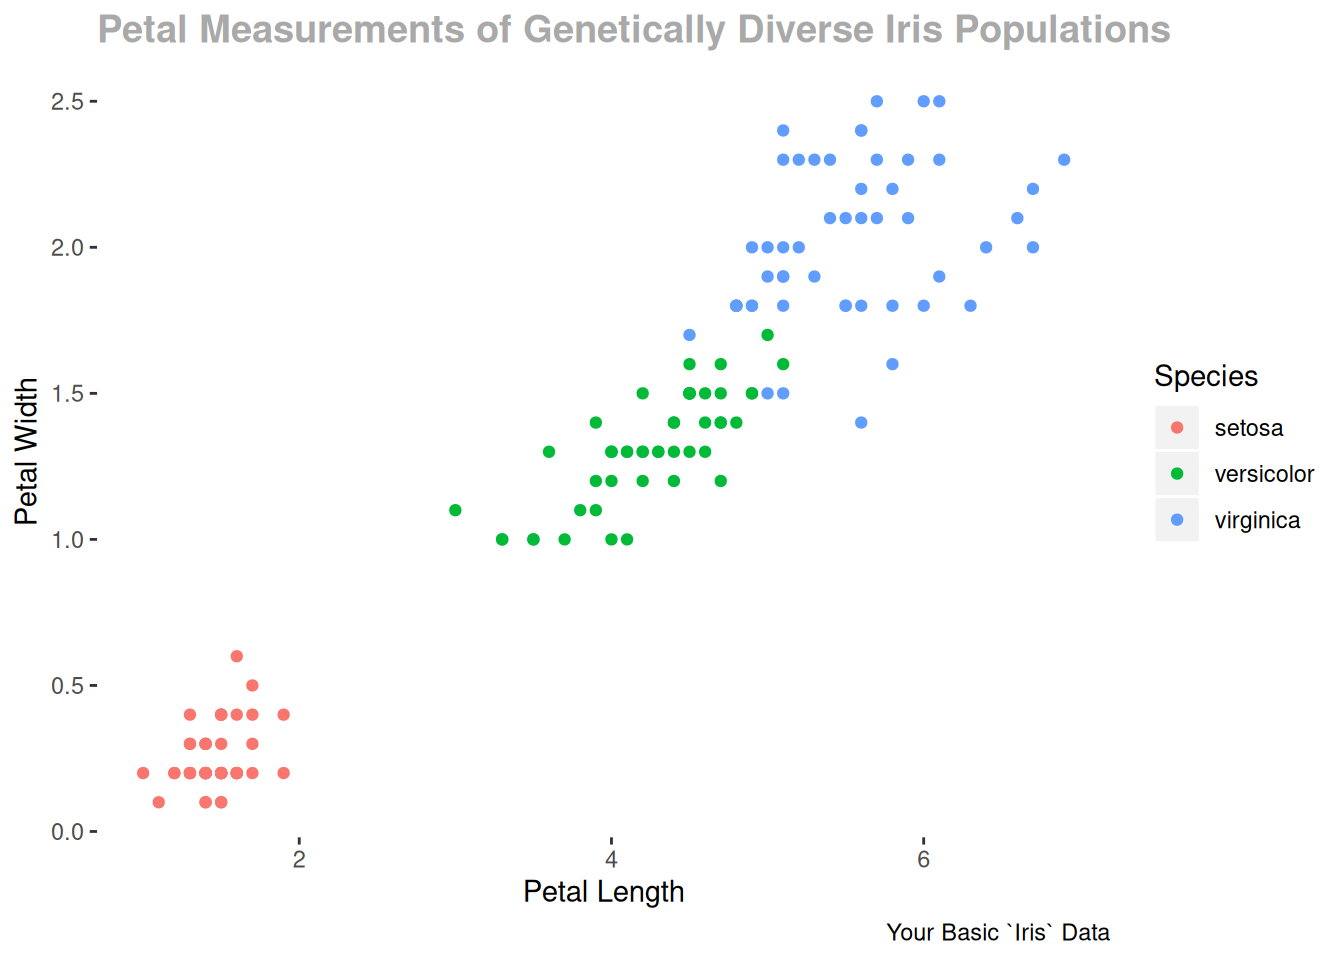
\includegraphics{Homework01_files/figure-latex/unnamed-chunk-2-1.pdf}

\begin{Shaded}
\begin{Highlighting}[]
\CommentTok{# Second graph}
\KeywordTok{ggplot}\NormalTok{(}\DataTypeTok{data =}\NormalTok{ Langren1644, }\KeywordTok{aes}\NormalTok{(}\DataTypeTok{x =}\NormalTok{ Longitude, }\DataTypeTok{y =}\NormalTok{ Latitude)) }\OperatorTok{+}\StringTok{ }
\StringTok{  }\KeywordTok{geom_point}\NormalTok{(}\KeywordTok{aes}\NormalTok{(}\DataTypeTok{color =} \DecValTok{1}\NormalTok{))}
\end{Highlighting}
\end{Shaded}

\includegraphics{Homework01_files/figure-latex/unnamed-chunk-2-2.pdf}

\begin{Shaded}
\begin{Highlighting}[]
\CommentTok{# Third graph}
\CommentTok{# update this code with changes you made in the second graph as well}
\KeywordTok{ggplot}\NormalTok{(}\DataTypeTok{data =}\NormalTok{ Langren1644, }\KeywordTok{aes}\NormalTok{(}\DataTypeTok{x =}\NormalTok{ Longitude, }\DataTypeTok{y =}\NormalTok{ Latitude)) }\OperatorTok{+}\StringTok{ }
\StringTok{  }\KeywordTok{geom_point}\NormalTok{(}\KeywordTok{aes}\NormalTok{(}\DataTypeTok{color =} \DecValTok{1}\NormalTok{))}
\end{Highlighting}
\end{Shaded}

\includegraphics{Homework01_files/figure-latex/unnamed-chunk-2-3.pdf}

\begin{Shaded}
\begin{Highlighting}[]
\CommentTok{# Fourth graphic}
\CommentTok{# update this code with changes you made in the third graphic}
\KeywordTok{ggplot}\NormalTok{(}\DataTypeTok{data =}\NormalTok{ Langren1644, }\KeywordTok{aes}\NormalTok{(}\DataTypeTok{x =}\NormalTok{ Longitude, }\DataTypeTok{y =}\NormalTok{ Latitude)) }\OperatorTok{+}\StringTok{ }
\StringTok{  }\KeywordTok{geom_point}\NormalTok{(}\KeywordTok{aes}\NormalTok{(}\DataTypeTok{color =} \DecValTok{1}\NormalTok{)) }\OperatorTok{+}\StringTok{ }
\StringTok{  }\KeywordTok{geom_text}\NormalTok{(}\KeywordTok{aes}\NormalTok{(}\DataTypeTok{label =}\NormalTok{ Name), }\DataTypeTok{hjust =} \FloatTok{-0.05}\NormalTok{, }
    \DataTypeTok{vjust =} \FloatTok{-0.05}\NormalTok{, }\DataTypeTok{angle =} \DecValTok{-90}\NormalTok{)}
\end{Highlighting}
\end{Shaded}

\includegraphics{Homework01_files/figure-latex/unnamed-chunk-2-4.pdf}

\begin{itemize}
\item
  (5 points) In the first graph, update the graphic by using light blue
  (\texttt{"lightblue"}) to color the bars, and add an appropriate
  title, and (if you want) add a caption specifying the source of the
  data (use the approach in Lab 01 to do this).
\item
  (10 points) In the second graph we observe a scatter plot of Longitude
  vs Latitude. Use \texttt{help(Langren1644)} to read about the
  variables in the \texttt{Langren1644} data, and briefly describe the
  axis of the plot. Next we will modify the plot. First, replace the
  variable \texttt{Latitude} with \texttt{Year}. In order to get more
  information to the plot we want to color the points in the scatter
  plot according to which country does the longitude estimate comes
  from. To achieve this use the \texttt{color} argument of the aesthetic
  mappings function \texttt{aes} and set it equal to the variable
  associated with country of origin (may need to look at
  \texttt{help(Langren1644)} again).
\item
  (5 points) With the third graph make it have the same updates of the
  second graph. To sqeeze in some more information, change the shape of
  the points according to the \textbf{source} of longitudinal
  measurement used. To do so mimic what you did in with the
  \texttt{color} parameter in \texttt{aes}, but this time do
  \texttt{aes(color\ =\ ...,\ shape\ =\ Source)}. Next, we will add a
  vertical line, indicating the true longitudinal distance between
  Toledo and Rome. To find this distance you can use Google, or
  \texttt{help(Langren1644)}. To add the vertical line we use
  \texttt{+\ geom\_vline(aes(xintercept\ =\ \_))} right after the
  \texttt{geom\_point(...)} where you should subtitude \texttt{\_} with
  the longitudinal distance between Toledo and Rome.
\item
  (10 points) With the fourth graph make it have the same updates of the
  third graph. Add title to this fourth plot describing the two main
  variables (be brief) and a subtitle with any additional variables
  plotted. Based on the new plot answer the following questions:

  \begin{itemize}
  \tightlist
  \item
    Who gave the most precise estimate?
  \item
    Which country gave the most accurate estimates?
  \item
    Is the oldest estimate the worst?
  \item
    Which source seems more accurate?
  \end{itemize}
\end{itemize}

\begin{center}\rule{0.5\linewidth}{\linethickness}\end{center}

\begin{center}\rule{0.5\linewidth}{\linethickness}\end{center}

\hypertarget{problem-4}{%
\section{Problem 4}\label{problem-4}}

(23 points)

\textbf{Writing R Functions and Working with Vectors}:

Read section 5 of Wasserman's R Intro document on Canvas about writing
functions in R. Functions help us reuse code and enhance the
reproduciblity of our code.

\begin{enumerate}
\def\labelenumi{\alph{enumi}.}
\item
  (2 points) Write an R function called \texttt{abssum} that takes four
  inputs -- \texttt{a}, \texttt{b}, \texttt{x}, and \texttt{y} and
  returns the quantity \(ax + b|y|\).
\item
  (2 points) Test your function and demonstrate that it works for at
  least three different combinations of the parameters.
\item
  (2 points) Type \texttt{abssum(x\ =\ 1,\ y\ =\ 1)} into your code
  block. What happens when you only specify these two arguments? (Note:
  When knitting your document for submission, comment this line of code
  out, so that it does not produce an error.)
\item
  (2 points) Create a new function, \texttt{abssum2}, that has default
  values for \texttt{a\ =\ 1}, \texttt{b\ =\ 1}. Type
  \texttt{abssum2(x\ =\ 1,\ y\ =\ 1)} into your code block. What happens
  when you only specify the two arguments now?
\item
  (2 points) Type \texttt{1:10} at the command line in \texttt{R}. What
  happens?
\item
  (2 points) What happens when you call the function with the following
  input: \texttt{abssum2(x\ =\ 1:10,\ y\ =\ 1:10)}. Why does this
  happen?
\item
  (8 points) Use \texttt{help(rnorm)} to learn about the function
  \texttt{rnorm} which generates normal random variables. Generate 5000
  independent standard normal random variables and assign them to
  \texttt{Z}. Repeat the same procedure and assign the new values to
  \texttt{W}. Type
  \texttt{plot(W,\ abssum2(x\ =\ Z,\ y\ =\ W),\ cex\ =\ .5,\ pch\ =\ 16,\ xlab\ =\ "W",\ ylab\ =\ "Z\ +\ \textbar{}W\textbar{}")}.
  Describe the graph that shows up, and explain why this happens.
\item
  (3 points) Use \texttt{ggplot2} to repeat the above plot. Don't worry
  whether the size of the points match the size of the points from part
  f.~Optionally include titles and label the axis for this problem.
  (hint: assuming \texttt{W} and \texttt{Z} exist, you can create a data
  frame with
  \texttt{D\ \textless{}-\ data.frame(V1\ =\ W,\ V2\ =\ abssum2(x\ =\ Z,\ y\ =\ W))};
  then use the knowledge from the commented code of Lab 01 and Homework
  01, Problem 3 part e).
\end{enumerate}

\begin{center}\rule{0.5\linewidth}{\linethickness}\end{center}

\begin{center}\rule{0.5\linewidth}{\linethickness}\end{center}

\hypertarget{problem-5}{%
\section{Problem 5}\label{problem-5}}

(5 points)

\textbf{Enroll in Piazza for 36-315}:

All questions about homeworks, labs, the lab exam, projects, course
material, etc should be posted to the discussion board on Piazza.

\begin{enumerate}
\def\labelenumi{\alph{enumi}.}
\item
  (1 points) If you're not already signed up, enrolled in our Piazza
  course \href{https://piazza.com/cmu/fall2018/36315}{here}.
  Alternatively, you can sign-up and view Piazza via the class Canvas.
  \textbf{IT IS CRITICAL THAT YOU ENROLL IN THE COURSE ON PIAZZA.}
  Important course discussion and information will only be distributed
  via Piazza. You are responsible for understanding all content that is
  posted to Piazza.
\item
  (0 points) On the course Piazza page, in the top-right corner, click
  the Settings gear/wheel icon. Under Account \& Email Settings, click
  Edit Email Notifications. I recommend choosing Real Time for both
  parts and checking the ``Automatically follow every question and
  note'' checkbox.
\item
  (2 points) Write the following sentence: ``I certify that I understand
  that I am responsible for reading and understanding all material and
  content posted on the course Piazza page.''
\item
  (2 points) Write the following sentence: ``I certify that I will not
  abuse the use of anonymous posting on the course Piazza page.''
\end{enumerate}

\begin{center}\rule{0.5\linewidth}{\linethickness}\end{center}

\begin{center}\rule{0.5\linewidth}{\linethickness}\end{center}

\hypertarget{problem-6}{%
\section{Problem 6}\label{problem-6}}

(5 points)

\textbf{Consent to Use Lab Solutions}:

If you do very well on a lab, we would like to post your solutions for
that lab assignment to Canvas for other students to see. Posted
solutions will, of course, be anonymized, so that other students will
not know that the solutions are yours. We will not post homework or lab
exam solutions to Canvas.

You are welcome to opt out of this if you want to. Just answer the
following question: Do you consent to having your (anonymized) lab
solutions posted to Canvas? (Just type ``Yes'', or ``No''.)

(You will receive 5 points regardless of what you answer -- we just need
to know ahead of time!)


\end{document}
